\documentclass[11pt]{article}

% ---------------------------------------------------------------------------
% Working draft --- LD-aware outlier-region detection (LDscnR C-score).
% Assembled during the analysis sessions. The two sections drafted in full
% below (structure-aware null; detectability) are the most developed; the
% remaining sections are skeletons to be filled in. Figures are referenced
% from ./figures/ --- drop the generated PNGs there.
%
% Compile:  pdflatex ld_aware_outlier_regions ; bibtex ld_aware_outlier_regions ;
%           pdflatex (x2)
% ---------------------------------------------------------------------------

\usepackage[margin=1in]{geometry}
\usepackage{amsmath,amssymb}
\usepackage{graphicx}
\graphicspath{{figures/}}
\usepackage[round]{natbib}
\usepackage{booktabs}
\usepackage{longtable}
\usepackage{microtype}
\usepackage[hidelinks]{hyperref}
\usepackage{xcolor}
\newcommand{\todo}[1]{\textcolor{red}{[\textsc{todo}: #1]}}
\newcommand{\tauc}{\ensuremath{\tau_C}}
\newcommand{\lmin}{\ensuremath{\ell_{\min}}}

\title{Leveraging local linkage disequilibrium to detect and calibrate
outlier regions in genome scans}
\author{\todo{author list}}
\date{\today}

\begin{document}
\maketitle

\begin{abstract}
\todo{abstract} We describe an outlier-region detection method for genome scans
that exploits the tendency of true selection signals to be locally
linkage-disequilibrium (LD) supported: a causal variant drags a block of
correlated markers with it, so genuine signal appears as clusters of
consistently prioritised markers rather than as isolated peaks. Each marker is
assigned a consistency score (the \emph{C-score}) that integrates two nuisance
parameters --- the LD window and the local-LD quantile --- at a fixed
false-discovery level; markers are then clustered into regions by LD, and
regions are retained by a size filter. We calibrate the detection threshold with
a \emph{structure-aware null} that requires no per-locus permutation, and we
provide a \emph{detectability} diagnostic that flags datasets in which structure,
rather than signal, dominates. \todo{results one-liner}
\end{abstract}

\section{Introduction}
\todo{Introduction: genome scans for selection / genotype--environment
association; the problems of population and spatial structure, of per-locus
multiple testing, and of over-interpreting structure artifacts; the LD-support
premise; overview of contributions.}

\section{Methods}

\subsection{The consistency (C-)score}
\label{sec:cscore}

The method rests on a single premise: selection locally inflates linkage
disequilibrium. A sweep, or a barrier to gene flow, raises LD in the
neighbourhood of its target, so a true signal is not an isolated peak but a
\emph{block} of mutually correlated markers. ``LD-supported'' and ``clustered''
are therefore not two separate properties but the same footprint of locally
elevated LD, seen per-marker and per-region. The C-score turns this premise into
a per-marker statistic by asking how \emph{consistently} a marker is both
prioritised by local LD and statistically associated with the focal variable.

\paragraph{Local-LD statistic.}
For each chromosome we fit an LD-decay curve to the pairwise $r^2$ between markers
as a function of physical distance, with decay rate $a$. For a relative-LD level
$\rho \in (0,1)$ this curve defines a neighbourhood of half-width
$d(\rho) = \rho / [\,a(1-\rho)\,]$: a small $\rho$ probes a tight window and a
large $\rho$ a broad one. The local-LD statistic of marker $j$ at scale $\rho$ is
the median $r^2$ between $j$ and the other markers within $d(\rho)$,
\begin{equation}
  w_j(\rho) \;=\; \operatorname{median}\bigl\{\, r^2_{jk} \;:\; |x_j - x_k| \le d(\rho) \,\bigr\},
\end{equation}
where $x_j$ is the position of marker $j$. It is large for markers sitting inside
a dense LD block and small for isolated markers.

\paragraph{Consistency over the two nuisance parameters.}
Turning $w(\rho)$ into a set of ``local-LD candidates'' requires two choices with
no canonical value: the window scale $\rho$ and a stringency quantile
$q^* \in [0,1]$ above which a marker counts as a candidate. Rather than fix
either, we sweep both. For a cell $(\rho, q^*)$ the candidate set is
\begin{equation}
  \mathcal{C}(\rho, q^*) \;=\; \bigl\{\, j : w_j(\rho) \ge Q_{q^*}\!\left[\,w(\rho)\,\right] \,\bigr\},
\end{equation}
where $Q_{q^*}$ is the empirical $q^*$-quantile of the local-LD statistic. Within
the candidates---and only within them, so the multiple-testing burden is carried
by the candidate set rather than the whole genome---we control the false-discovery
rate of the association $p$-values \citep{benjamini1995controlling}: a marker is a
\emph{hit} in cell $(\rho, q^*)$ if it is a candidate and its
Benjamini--Hochberg-adjusted $p$-value \emph{among the candidates} is below a
level $\alpha$. The C-score of marker $j$ is the fraction of cells in which it is
a hit,
\begin{equation}
  C_j \;=\; \frac{1}{|R|\,|Q|} \sum_{\rho \in R}\ \sum_{q^* \in Q}
        \mathbb{1}\!\left[\, j \in \mathcal{C}(\rho, q^*)\ \text{and}\
        \mathrm{BH}\text{-}q_j(\rho, q^*) < \alpha \,\right] \;\in\; [0,1],
  \label{eq:cscore}
\end{equation}
evaluated over a grid $R$ of window scales and a grid $Q$ of stringency
quantiles. A marker scores highly only if it is repeatedly \emph{both}
LD-prioritised \emph{and} significant across scales and stringencies; a marker
that is significant but not LD-supported (an isolated peak), or LD-supported but
not significant, scores low. The C-score thus operationalises the LD-support
premise directly, without committing to a single LD scale or candidate threshold.

\paragraph{Which parameters to sweep, and which to fix.}
The two swept parameters, $\rho$ and $q^*$, are natural $[0,1]$ quantities, so
integrating over them is assumption-free---the C-score privileges no single LD
scale or candidate stringency. The false-discovery level $\alpha$, by contrast,
has no natural range, so we do not sweep it but fix it at the conventional
$\alpha = 0.05$. Fixing $\alpha$ is defensible because any resulting
miscalibration---an anticonservative test inflating the number of hits---raises
the score of null and true markers alike, and is therefore \emph{priced in} by
the structure-aware threshold calibration of Section~\ref{sec:null}: an inflated
$p$-value distribution raises the null C-score as much as the observed one, and
the region-level false-discovery ratio moves the threshold accordingly. The input
to Eq.~\ref{eq:cscore} is a vector of per-marker association $p$-values and may
come from any association test; we use EMMAX \citep{kang2010variance} and LFMM
\citep{caye2019lfmm}.

\subsection{An LD-aware kinship for the association scan}
\label{sec:grm}

EMMAX controls for relatedness and population structure through a genomic
relationship matrix (GRM) estimated from a set of markers, and the choice of that
set matters more than is usually acknowledged. Two failure modes bracket the
problem. If the GRM \emph{includes} the very regions under selection, it absorbs
their association signal into the ``structure'' it corrects for, and those regions
go silent---an over-correction that is \emph{regional}. If instead the GRM is
built from too many mutually correlated markers, it is over-parameterised and
\emph{deflates} the whole test-statistic distribution---an over-correction that is
\emph{global}. The two are not interchangeable, and, crucially, they are not
equally visible.

\paragraph{Pruning on the local-LD statistic.}
We build the GRM from LD-\emph{independent} markers, reusing the same local-LD
statistic $w_j(\rho)$ of Eq.~\ref{eq:cscore}'s candidate step (evaluated at a
broad reference scale): markers whose local-LD support falls below a cutoff,
$\{\, j : w_j < \omega \,\}$, form the kinship. Pruning on $w_j$ rather than on
physical distance or a fixed marker count is what makes the kinship robust,
because $w_j$ is exactly the quantity the method already expects to be elevated
at a signal:
\begin{itemize}
  \item \textbf{If an outlier region has high $w_j$}---the expected case, since
    selection locally inflates LD (the premise of Section~\ref{sec:cscore}), and
    inversions and low-recombination blocks carry extended LD---then $w_j$-pruning
    \emph{excludes} it from the kinship, so the GRM cannot absorb its signal.
  \item \textbf{If an outlier region has low $w_j$}---a point signal in a weakly
    linked genome---then the same rule \emph{keeps} it; but a marker with little
    local LD carries almost no structure and is nearly inert in the kinship, so no
    harm is done.
  \item \textbf{As a by-product}, pruning the high-$w_j$ markers removes the large
    low-recombination LD blocks whose extended correlations would otherwise
    dominate the relatedness estimate---the GRM's worst confounders are discarded
    for free.
\end{itemize}
$w_j$-pruning therefore either removes the signal from the kinship or harmlessly
ignores it, and in every case removes the confounding LD blocks: it cannot corrupt
the kinship on the signal side.

\paragraph{Setting the stringency by the inflation factor.}
This leaves only the \emph{global} failure mode---over-parameterisation---to
control, and the genomic inflation factor
$\lambda = \operatorname{median}(\chi^2_{\text{obs}}) /
\operatorname{median}(\chi^2_{\text{null}})$ \citep{devlin1999genomic} measures it
directly: a GRM built from too many markers drives $\lambda$ below one. We
therefore set the pruning cutoff $\omega$ by $\lambda$, tightening it (retaining
fewer, more independent markers, which weakens the correction and raises
$\lambda$) until $\lambda \ge 1$---the largest, most powerful marker set that is
not yet deflated. It is important that $\lambda$ is used only for this one job.
The regional failure mode is invisible to it: absorbing a single high-LD region
leaves the median marker---which is not under selection---untouched, so $\lambda$
barely moves even as the signal is erased. $\lambda \approx 1$ is thus a valid
guard against global deflation but blind to regional absorption; it is the
$w_j$-pruning that forecloses the regional mode by construction, and $\lambda$
that then trims the remaining excess. Because the residual structure a
$\lambda \ge 1$ kinship leaves behind is exactly what the structure-aware null of
Section~\ref{sec:null} is designed to absorb, the division of labour is clean: the
kinship must only avoid deflation, and the null calibrates whatever structure it
leaves.

\subsection{Clustering C-score outliers into regions}
\label{sec:cluster}

An outlier set is obtained by thresholding the C-score, $\{\, j : C_j \ge \tauc \,\}$,
and the retained markers are grouped into regions. Because a true signal is an
LD-supported block rather than a single peak (Section~\ref{sec:cscore}), we group
by \emph{linkage} rather than by physical proximity alone: two markers on the same
chromosome are joined when their $r^2$ exceeds a threshold, a region is a
connected component of the resulting graph, and a component is split wherever its
members straddle a large physical gap.

\paragraph{Linkage threshold.}
The $r^2$ join threshold is decay-relative and self-calibrates per chromosome. For
a chromosome whose fitted LD-decay curve has background (asymptotic) LD $b$ and
short-range $r^2$ $c$, and a relative-LD level $\rho_{\mathrm{ld}} \in [0,1]$,
markers $j$ and $k$ are joined when
\begin{equation}
  r^2_{jk} \;\ge\; b + (c - b)\,(1 - \rho_{\mathrm{ld}}).
\end{equation}
As $\rho_{\mathrm{ld}} \to 1$ the threshold approaches the background $b$ and
almost everything links; as $\rho_{\mathrm{ld}}$ decreases the threshold rises
toward $c$ and only tightly linked markers join. Lowering $\rho_{\mathrm{ld}}$
therefore resolves a broad region into its component haplotype blocks by LD---the
property that lets a genuinely high-LD region (an inversion) remain a single unit
while an adjacent, looser cluster is separated, which a fixed $r^2$ cutoff cannot
do.

\paragraph{Regions and the distance cap.}
A region is a connected component (single linkage) of the thresholded $r^2$ graph
within a chromosome, split wherever consecutive members, ordered by position, are
more than a hard distance cap $d_{\mathrm{cap}}$ (default $500$~kb) apart. A
region's extent is bounded by this cap rather than by LD decay because its
footprint is set by selection and local recombination, not by background LD:
long-range $r^2$ is the rule inside inversions, so a decay-derived distance would
fragment a single inversion into many pieces. (The cap may optionally be made
decay-relative, $d(\rho_d) = \rho_d / [\,a(1-\rho_d)\,]$ capped at
$d_{\mathrm{cap}}$, but the hard cap is the default.) Because the linkage graph is
built once over the candidate universe $\{\, j : C_j > 0 \,\}$, any thresholded
subset can be clustered by graph lookup with no further genotype access; a strong
single-marker hit and a marker prioritised by local LD at the same locus
consequently fall in the same region and are counted once.

\paragraph{The size filter, and the two clustering roles.}
Regions with fewer than \lmin\ markers are discarded. \lmin\ is not part of the
C-score but a post-filter, and it is the principal false-positive control:
structure noise produces small, scattered clusters, whereas a selected locus drags
a block of linked markers, so a size floor removes the former far faster than the
latter. It is useful to distinguish the two clustering roles.
$\rho_{\mathrm{ld}}$ and $d_{\mathrm{cap}}$ are \emph{boundary} controls---they
decide where one region ends and thus set each region's shape and extent---whereas
\lmin\ is a \emph{removal} control that decides which regions are reported. They
compose but are not interchangeable: tightening the boundary controls sheds
loosely linked or distant markers off a block, but a shed piece does not vanish,
it becomes its own small region, and only \lmin\ removes it. The calibration of
\tauc\ and \lmin\ is the subject of Section~\ref{sec:null}, and the diagnostic for
when this procedure can resolve signal at all is the subject of
Section~\ref{sec:detect}.

% ===========================================================================
\subsection{Calibrating the detection threshold with a structure-aware null}
\label{sec:null}

Turning the continuous C-score into a set of outlier regions requires a
threshold, \tauc, and a minimum region size, \lmin. Rather than deriving a
per-locus significance level---which, under population or spatial structure,
would require resolving the null \emph{tail} to genome-wide-significant
precision and hence thousands of structure-preserving permutations per
locus (prohibitive for latent-factor models such as LFMM)---we calibrate a
single \emph{region-level} operating point against a structure-aware null.

We generate $B$ surrogate phenotypes that retain the autocorrelation structure
of the data but are orthogonal to the focal environment. Each surrogate is drawn
as a Gaussian random field with covariance given by the genomic relationship
matrix $\mathbf{K}$ (or by a spatial kernel over sampling coordinates) and is
then residualised against the observed environment, so that it carries the same
structure while being decorrelated from the real signal. Re-running the
association test on each surrogate yields the null distribution of the C-score
and, after clustering, of the number of outlier regions. The threshold is set to
the smallest \tauc\ at which the region-level empirical false-discovery
rate---the mean number of surrogate regions of size $\ge\lmin$ divided by the
observed number---falls at or below a target level.

The number of regions produced under the null is a small count (typically zero
or a handful per surrogate), so a modest $B$ (50--100) resolves it, in contrast
to the thousands of permutations needed to place an individual locus beyond a
genome-wide significance threshold. We can afford this coarse null because the
multiple-testing burden is absorbed \emph{structurally} rather than by brute
force: the C-score already integrates each locus's evidence across the
$(\rho, q^*)$ grid with an internal false-discovery correction among local-LD
candidates, and the size filter \lmin\ removes the small clusters that dominate
false positives. The threshold \tauc\ therefore need only fall within a broad
safe region rather than on a knife-edge.

Indeed, \tauc\ and \lmin\ act as partially redundant false-positive controls
(Fig.~\ref{fig:heatmap}): raising either suppresses spurious regions. The
structure-aware null makes this explicit. Under the null, regions appear only as
\emph{small} clusters at low thresholds ($\lmin = 1$--$2$); for $\lmin \ge 3$ the
null is essentially silent across the whole range of \tauc. Averaged across
replicate simulations, the region of high precision--recall lies entirely within
this null-quiet zone, and the region in which the null produces false regions
coincides with the region of poorest performance. The null landscape---which is
obtainable \emph{without} knowledge of the truth---therefore identifies the safe
operating region directly. In practice this means the null does not have to
locate the optimal threshold; it has to locate the small-cluster ``danger
corner'' to avoid, after which \lmin\ does the residual false-positive work, and
how large \lmin\ must be scales with the noisiness (or baseline inflation) of the
underlying test.

For association tests that lack an inexpensive permutation null, we transfer the
calibrated threshold by genomic control on the C-scale
\citep{devlin1999genomic}: we compute the upper-tail quantile that \tauc\
occupies in the reference method's C distribution and read off the value at the
same quantile in the target method's distribution. This places the two methods
at a common false-positive anchor even when their raw score scales differ by an
order of magnitude.

\paragraph{Region-level empirical $p$-values and the choice of structure basis.}
The region-level FDR above sets a single genome-wide operating point; where
individual regions are of interest we additionally assign each its own empirical
$p$-value by \emph{location-matched} overlap. Scoring a region $R$ by its summed
C-mass $s_R = \sum_{j\in R} C_j$, we take as its $p$-value the fraction of
surrogates that produce a region overlapping $R$'s genomic span with mass at least
$s_R$, $p_R = \bigl(1 + \#\{b : s^{\mathrm{null}}_{b,R} \ge s_R\}\bigr)/(1+B)$.
This test is deliberately \emph{local}: a signal confined to part of the sampled
range need not be reproduced by a structure-preserving surrogate at its own locus,
so a genuinely range-restricted adaptation peak---one that a pooled, genome-wide
count-FDR would charge to structure---can still separate from the null here.

The surrogate basis encodes \emph{which} confounder is controlled, and this is a
modelling choice rather than a technicality. A \emph{genetic} basis, drawing the
surrogate from the same $\mathbf{K}$ the scan already conditions on, asks whether
the pipeline manufactures regions from structured-but-null data; because that
structure is absorbed by the correction, it is a \emph{specificity} control on the
method itself. A basis \emph{not} in the correction instead tests
\emph{attribution} against a named confounder: a smooth spatial kernel over
coordinates for a continuous environmental gradient, or a permutation of the
environmental labels among the discrete sampling units for a parallel, patchy
habitat contrast. The basis must match how the environment is actually
distributed. A mismatched basis---a smooth kernel imposed on a parallel
contrast---injects autocorrelation absent from both the environment and the
kinship correction, inflating the surrogate scans; the number of null peaks per
surrogate is a direct calibration check, a well-specified null producing at most a
handful while a mis-specified one rivals the observed scan in peak count. Crucially,
the \emph{location-matched} region test is robust to such global inflation: because
the excess null peaks are scattered, they rarely fall on any particular observed
locus, so an inflated basis does not erase regions indiscriminately but instead
flags only the loci it specifically and repeatedly reconstructs. This robustness is
a concrete advantage of a region-level location-matched null over a pooled
genome-wide count (Section~\ref{sec:threenull}).

\paragraph{Relationship to existing methods.}
Structure-aware surrogate nulls are well established outside genome scans.
Preserving spatial autocorrelation while breaking the association between two
spatially structured variables underlies the surrogate-lattice test of
\citet{deblauwe2012testing}, the generative surrogate maps of
\citet{burt2020generative}, eigenmode-rotation (``eigenstrapping'') approaches
\citep{eigenstrapping2024}, and the ``spin test'' \citep{alexanderbloch2018testing}
and Moran spectral randomization \citep{wagner2015generating} used in
neuroimaging and spatial ecology. Our contribution is to preserve \emph{genetic}
rather than purely spatial structure (via $\mathbf{K}$), to residualise against
the observed environment, and to use the resulting null to calibrate a
\emph{region-level} threshold for an LD-aware consistency score---an application,
to our knowledge, not previously made in selection or genotype--environment
scans.

% ===========================================================================
\subsection{Detectability: recognising when a genome scan can resolve signal}
\label{sec:detect}

Outlier scans return candidate loci whether or not the data contain resolvable
signal; on genomes where neutral structure dominates, the reported ``outliers''
are structure artifacts. A practical genome scan should therefore report whether
signal is separable from background \emph{at all}, so that saturated or
structure-dominated datasets can be flagged rather than over-interpreted.

The relevant contrast is between \emph{clear-peak} genomes, in which a small
number of loci rise sharply above an otherwise quiet background, and
\emph{saturated} genomes, in which signal is distributed across most of the
genome with no quiet background to serve as a reference. We summarise each
chromosome (or region) by its \emph{tail mass}---the number of markers exceeding
a fixed C-score---which measures the footprint of clustered high-scoring markers
and is robust to the isolated high-scoring markers that inflate simpler
statistics such as the per-chromosome maximum. Two truth-free quantities then
distinguish the regimes (Fig.~\ref{fig:detect}).

First, \emph{between-chromosome variation} in tail mass. In a detectable dataset
a few chromosomes tower over a near-zero bulk, giving a large ratio of the
maximum to the median tail mass (and a high coefficient of variation); in a
structure-dominated dataset every chromosome is similarly elevated and the ratio
collapses toward one. Second, the \emph{structure-aware null threshold} itself:
where signal is separable, the null falls silent at a moderate \tauc; where
structure dominates, the null remains as extreme as the observed data up to the
maximum threshold, so that any threshold that suppresses the structure also
suppresses everything.

In simulations these diagnostics agree and cleanly separate a gene-flow regime,
in which both indicate detectability and the method recovers the causal regions,
from a low-dispersal, structure-dominated regime, in which both indicate
non-detectability and even the best attainable precision--recall is near zero at
every threshold. The neutral chromosomes present by construction in the
simulations confirm the interpretation: their tail mass forms the quiet floor in
the detectable regime, whereas in the structure-dominated regime neutral
chromosomes reach tail masses as large as those carrying causal variants.

An important limitation follows. Where genuinely neutral chromosomes exist, they
define a floor against which the threshold can be calibrated directly; but on a
saturated genome no such floor exists---the apparently quiet chromosomes are
simply those with the weakest signal, and lowering the threshold eventually
recruits them all. On such genomes the threshold is unavoidably a
power/false-discovery-rate choice rather than a signal-versus-neutral
separation, and \lmin\ becomes the primary means of trading recall for
precision. Most published scans, however---recurrent freshwater adaptation in
stickleback \citep{kingman2021predicting}, sharp ecotype contrasts---occupy the
clear-peak end of this spectrum, where the diagnostics pass emphatically and
self-calibration is straightforward; the saturated case is the exception for
which the diagnostic is a safeguard.

\section{Results}
\todo{Simulation validation (C-score vs single-SNP alpha; PR-AUC); the
\tauc$\times$\lmin\ frontier; detectability across regimes; empirical
application (3sp; clear-peak contrast).}

\begin{figure}[t]
  \centering
  % \includegraphics[width=\linewidth]{heatmap_avg}
  \fbox{\parbox[c][0.32\linewidth][c]{\linewidth}{\centering\itshape
    Figure placeholder: mean truth precision$\times$recall (top) and mean number
    of regions under the structure-aware null (bottom) over the \tauc$\times$\lmin\
    grid, averaged across replicates. The high-PR ridge lies within the
    null-quiet zone; the null fires only in the small-cluster corner
    ($\lmin\le 2$, low \tauc).}}
  \caption{The \tauc$\times$\lmin\ operating landscape.}
  \label{fig:heatmap}
\end{figure}

\begin{figure}[t]
  \centering
  % 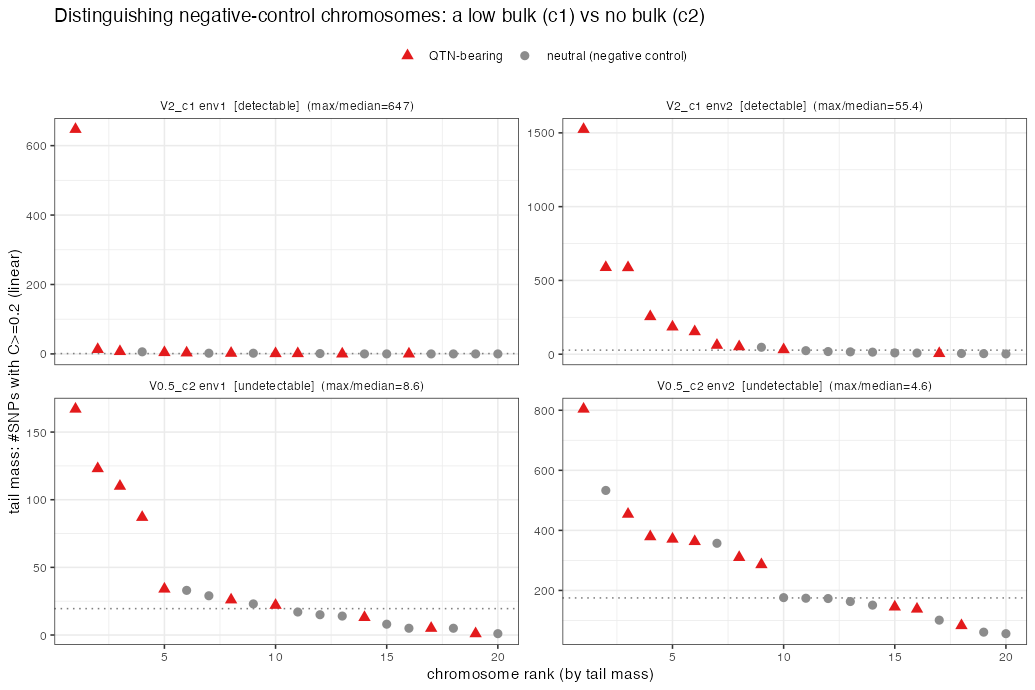
\includegraphics[width=\linewidth]{viz_negctrl_lin}
  \fbox{\parbox[c][0.32\linewidth][c]{\linewidth}{\centering\itshape
    Figure placeholder: per-chromosome tail mass, ranked, for a detectable
    (gene-flow) versus a structure-dominated (low-dispersal) regime. Detectable:
    a few chromosomes spike above a flat near-zero bulk. Undetectable: a gradual
    ramp with no floor.}}
  \caption{Detectability from the shape of the per-chromosome tail-mass profile.}
  \label{fig:detect}
\end{figure}

\subsection{Structure nulls on a stickleback marine--freshwater scan}
\label{sec:threenull}

We applied the scan to a three-spine stickleback (\textit{Gasterosteus aculeatus})
marine--freshwater dataset: $117$ individuals from $35$ populations spanning a
continental range (latitude $47$--$75^\circ$\,N). Single-SNP EMMAX resolves nothing
at $q \le 0.05$ (minimum $q \approx 0.06$), whereas the LD-aware C-score yields
$17$ outlier regions ($1729$ markers with $C > 0$) that recover the known
architecture---the chromosome-1 inversion, the \textit{Eda} region on
chromosome~4, and peaks on chromosomes 5, 7, 17 and 20. Holding this observed
region set fixed, we read it against four surrogate nulls that differ only in their
structure basis (Table~\ref{tab:threenull}); the median number of C-score peaks per
surrogate is the calibration diagnostic that interprets each.

The \emph{genetic} basis is silent. Drawn from the same kinship the scan conditions
on, it produces a median of \emph{zero} peaks per surrogate and not one null region
overlapping any of the $17$, which therefore all sit at the $p$-floor. This is the
specificity statement---the C-score-plus-clustering pipeline does not fabricate
regions from structured-but-null data, so the observed peaks are signal, not
clustering artifacts---but, because the surrogate is absorbed by the correction, it
cannot itself apportion signal between the ecotype contrast and population
structure.

The \emph{permutation} nulls do apportion it, and none of the $17$ regions is
reproduced. Shuffling the marine/freshwater label among all $35$ populations
(preserving population structure while breaking the ecotype--genotype link) rebuilds
no region at its own locus more than occasionally: every region clears $p < 0.05$
(median location-matched overlap $0.01$). A \emph{regional} refinement---permuting
the label only \emph{within} each of four localities, so that each locality's
ecotype composition is held fixed and only the within-region marine--freshwater
contrast is shuffled---is the sharper test of \emph{parallel} adaptation, since a
locus whose signal recurs within regions cannot be rebuilt by a within-region
shuffle. All $17$ regions again clear $p < 0.05$, the chromosome-1 inversion and
\textit{Eda} among them ($p = 0.015$ each). The permutation nulls thus place every
region above population structure and, specifically, above the within-region
reshuffling that would expose a merely between-region (clinal) signal. We note that
a \emph{pooled} genome-wide count-FDR against the same permutation null is far
blunter---dominated by the rare permutation that lights up a whole structured block,
it retains essentially one region---so the location-matched test is what makes these
nulls usable.

The \emph{spatial} basis is the informative outlier. A Gaussian random field over
the sampling coordinates is globally \emph{inflated}: it emits a median of $792$
peaks per surrogate, against $1729$ observed, because a smooth field carries
autocorrelation the genetic kinship does not remove---the peak-count diagnostic
($792 \gg 0$) flags this directly. Yet the location-matched region test is
\emph{robust} to that inflation: the excess null peaks are scattered, so they rarely
fall on a given locus, and $15$ of the $17$ regions still clear $p < 0.05$. The two
exceptions are precisely the chromosome-1 inversion ($p = 0.26$, overlap $0.43$) and
\textit{Eda} ($p = 0.44$, overlap $0.44$)---the two large-effect loci whose
differentiation is strongly clinal, so that a smooth spatial surrogate reconstructs
them. Critically, these are the same two loci the \emph{regional} permutation
certifies as within-region parallel signals: the spatial and regional nulls
\emph{disagree} exactly at the inversion and \textit{Eda}, and they disagree because
the spatial basis is the wrong model for a parallel contrast. Marine--freshwater
divergence recruits the same freshwater alleles at independent, scattered sites; a
smooth field cannot represent that and so mis-attributes the inversion and
\textit{Eda} to geography, whereas the within-region permutation---matched to the
parallel structure---shows their signal recurs within localities. On the
simulations, where the environment genuinely is a smooth gradient, the identical
spatial null is well calibrated and recovers the causal regions
(Section~\ref{sec:null}); here it errs only where the basis does not match the data,
and the mismatch is diagnosable both from the peak count and from the disagreement
with the correctly specified null.

Together the nulls give a specificity-then-attribution reading. The genetic null
certifies that the regions are real method output; the permutation nulls place all
$17$ above population structure and above the within-region reshuffling that a
purely clinal signal could not survive; and the spatial null, read against the
regional one, both illustrates the basis-matching principle and demonstrates that
the location-matched region test is robust to a mis-specified, inflated null.

\begin{table}[h]
  \centering
  \small
  \begin{tabular}{llcccc}
    \hline
    null (basis) & controls for & med.\ null & Chr1 inv. & \textit{Eda}/Chr4 & regions \\
                 &              & peaks/surr. & $p$ & $p$ & $p<0.05$ \\
    \hline
    genetic (MVN, $\mathbf{K}$)        & specificity (method)     & $0$   & $0.010^{\dagger}$ & $0.010^{\dagger}$ & $17/17$ \\
    perm., global (among pops)         & population structure     & $6$   & $0.015$           & $0.015$           & $17/17$ \\
    perm., regional (within locality)  & within-region parallel   & $6$   & $0.015$           & $0.015$           & $17/17$ \\
    spatial (GP kernel)                & spatial autocorrelation  & $792$ & $0.264$           & $0.443$           & $15/17$ \\
    \hline
  \end{tabular}
  \caption{Four structure nulls on the stickleback scan (observed: $1729$ C-score
  markers forming $17$ regions). The median number of C-score peaks per surrogate is
  the null-calibration diagnostic: the genetic basis is silent (a specificity
  control on the method), the permutation bases fire only occasionally, and the
  spatial basis is globally inflated ($792 \gg 0$)---a smooth field mismatched to a
  parallel habitat contrast. Despite that inflation the location-matched region test
  retains $15/17$ regions under the spatial null; the two it does not are the
  strongly clinal chromosome-1 inversion and \textit{Eda}, which the within-locality
  permutation nonetheless certifies as within-region parallel signals. Region
  $p$-values are location-matched overlap tests (Section~\ref{sec:null}).
  $^{\dagger}$~$p$-floor $1/(1+B)$ at $B = 100$ (genetic); the permutation and
  spatial nulls use $B = 200$ (floor $0.005$).}
  \label{tab:threenull}
\end{table}

\subsection{External validation against an independent dataset}
\label{sec:kingman}

The structure nulls are negative controls: they establish that the regions are not
method artifacts (genetic) and that they exceed population, within-region and
spatial structure (the permutation and spatial nulls). What no within-sample null
can do is confirm that a region is \emph{biologically} real rather than merely
non-spurious. Independent recovery of the same loci in a separate dataset and
pipeline is the complementary positive control.

We compared the $17$ regions against the recurrent marine--freshwater EcoPeaks of
\citet{kingman2021predicting}, which come from independent cohorts (a global panel
and a North-Eastern Pacific panel), an independently implemented SNP-based ecotype
test, and a different genome assembly (gasAcu1-4, lifted to common coordinates).
The regions overlap the global-specific EcoPeaks $19.5\times$ more than a
within-chromosome rotation null ($5/17$ regions, $p = 5\times10^{-4}$, $B = 2000$)
and the Pacific-specific set $2.4\times$ ($p = 0.04$). Three regions coincide with
\emph{both} cohorts' specific peaks (Fig.~\ref{fig:venn}), among them the
chromosome-1 inversion---recovered by four independent routes: the EMMAX and the
LFMM 3sp scans, the published global EcoPeak (SNP $p = 4.5\times10^{-15}$), and the
strongest suggestive peak in the geographically matched North-European cohort.
\textit{Eda} likewise falls on a strong EcoPeak in both cohorts
($p \approx 10^{-14}$); as a weak four-SNP cluster it is a detection-margin signal,
present at $\ell_{\min} = 3$ but lost at $\ell_{\min} = 10$, so its recovery is real
but parameter-sensitive.

Three points keep the comparison honest. First, the overlap is far stronger against
this tight $17$-region set than against a looser $\ell_{\min} = 10$ clustering ($40$
regions over $21$\,Mb), where dilution drops the global-specific overlap to
$1.4\times$ ($p = 0.33$)---the region set, not just the data, matters. Second, the
signal is geographically coherent. A rank-based enrichment of low Kingman
$p$-values inside the $17$ regions is strongest for the ocean-basin-matched
Northern-European cohort ($34\times$ among the top $1\%$ of SNPs, $p = 0.002$) and
remains high for the global ($26\times$, $p = 0.004$) and North-Eastern Pacific
($18\times$, $p = 0.002$) cohorts; independently, $5$ of the $41$ Northern-European
suggestive peaks fall inside the regions ($15\times$, $p = 2\times10^{-4}$). Since
the 3sp panel is North-European Atlantic, the matched cohort giving the strongest
signal is the expected pattern, and it locates the residual weakness of the raw
published-peak overlap in geography rather than in the method. Third, the force of
the result is the \emph{convergence} of a negative and a positive control---the
structure nulls show the peaks are not artifacts, and the independent data show they
mark real, recurrent adaptation loci; neither line alone would carry the claim.

The scan and clustering threshold trade specificity for sensitivity, and the
Kingman comparison exposes the trade cleanly. The tight EMMAX set used above ($17$
regions, $1.2$\,Mb) is the specific end---$19.5\times$ global-specific overlap---and
every one of its regions is corroborated by at least one other set
(Table~\ref{tab:crossset}). Running the LFMM scan at the same $\ell_{\min} = 3$
instead casts a wide net ($136$ regions, $37$\,Mb, $\sim\!10\%$ of the genome): it
recovers more EcoPeaks in absolute terms ($9$ global- and $28$ Pacific-specific
regions) but at much weaker per-region enrichment ($1.9\times$ and $1.3\times$), and
$78$ of its $136$ regions are singletons found by no other set. Raising $\ell_{\min}$
to $10$ removes regions from both scans without adding any (the $\ell_{\min}=10$
sets are strict subsets of the $\ell_{\min}=3$ sets). The tight EMMAX set is thus
the natural primary, with LFMM a sensitive complement---and the cross-set table is
itself a robustness statement: the loci recovered by several method/threshold
combinations and by Kingman (the chromosome-1 inversion in all six columns; Chr5:$2.5$
and Chr20:$0.18$ in five) are the most secure.

A few regions overlap a Pacific-specific but not a global-specific EcoPeak---for
example Chr4:$25.7$ and Chr5:$2.5$ in the EMMAX set, and many more in the broader
LFMM set---loci flagged as recurrent marine--freshwater targets in the Pacific and
independently recovered in the Atlantic 3sp panel, i.e.\ candidate cases of
cross-basin parallel adaptation at loci the global analysis does not single out. The
\emph{count} of such Pacific-only overlaps should not be over-interpreted: the
Pacific-specific set covers roughly seven times more genome than the global-specific
set, and on the coverage-adjusted rotation-null scale the global-specific fold is in
fact the higher of the two. It is the identity of the individual loci, not the raw
tally, that is informative.

\begin{figure}[t]
  \centering
  % 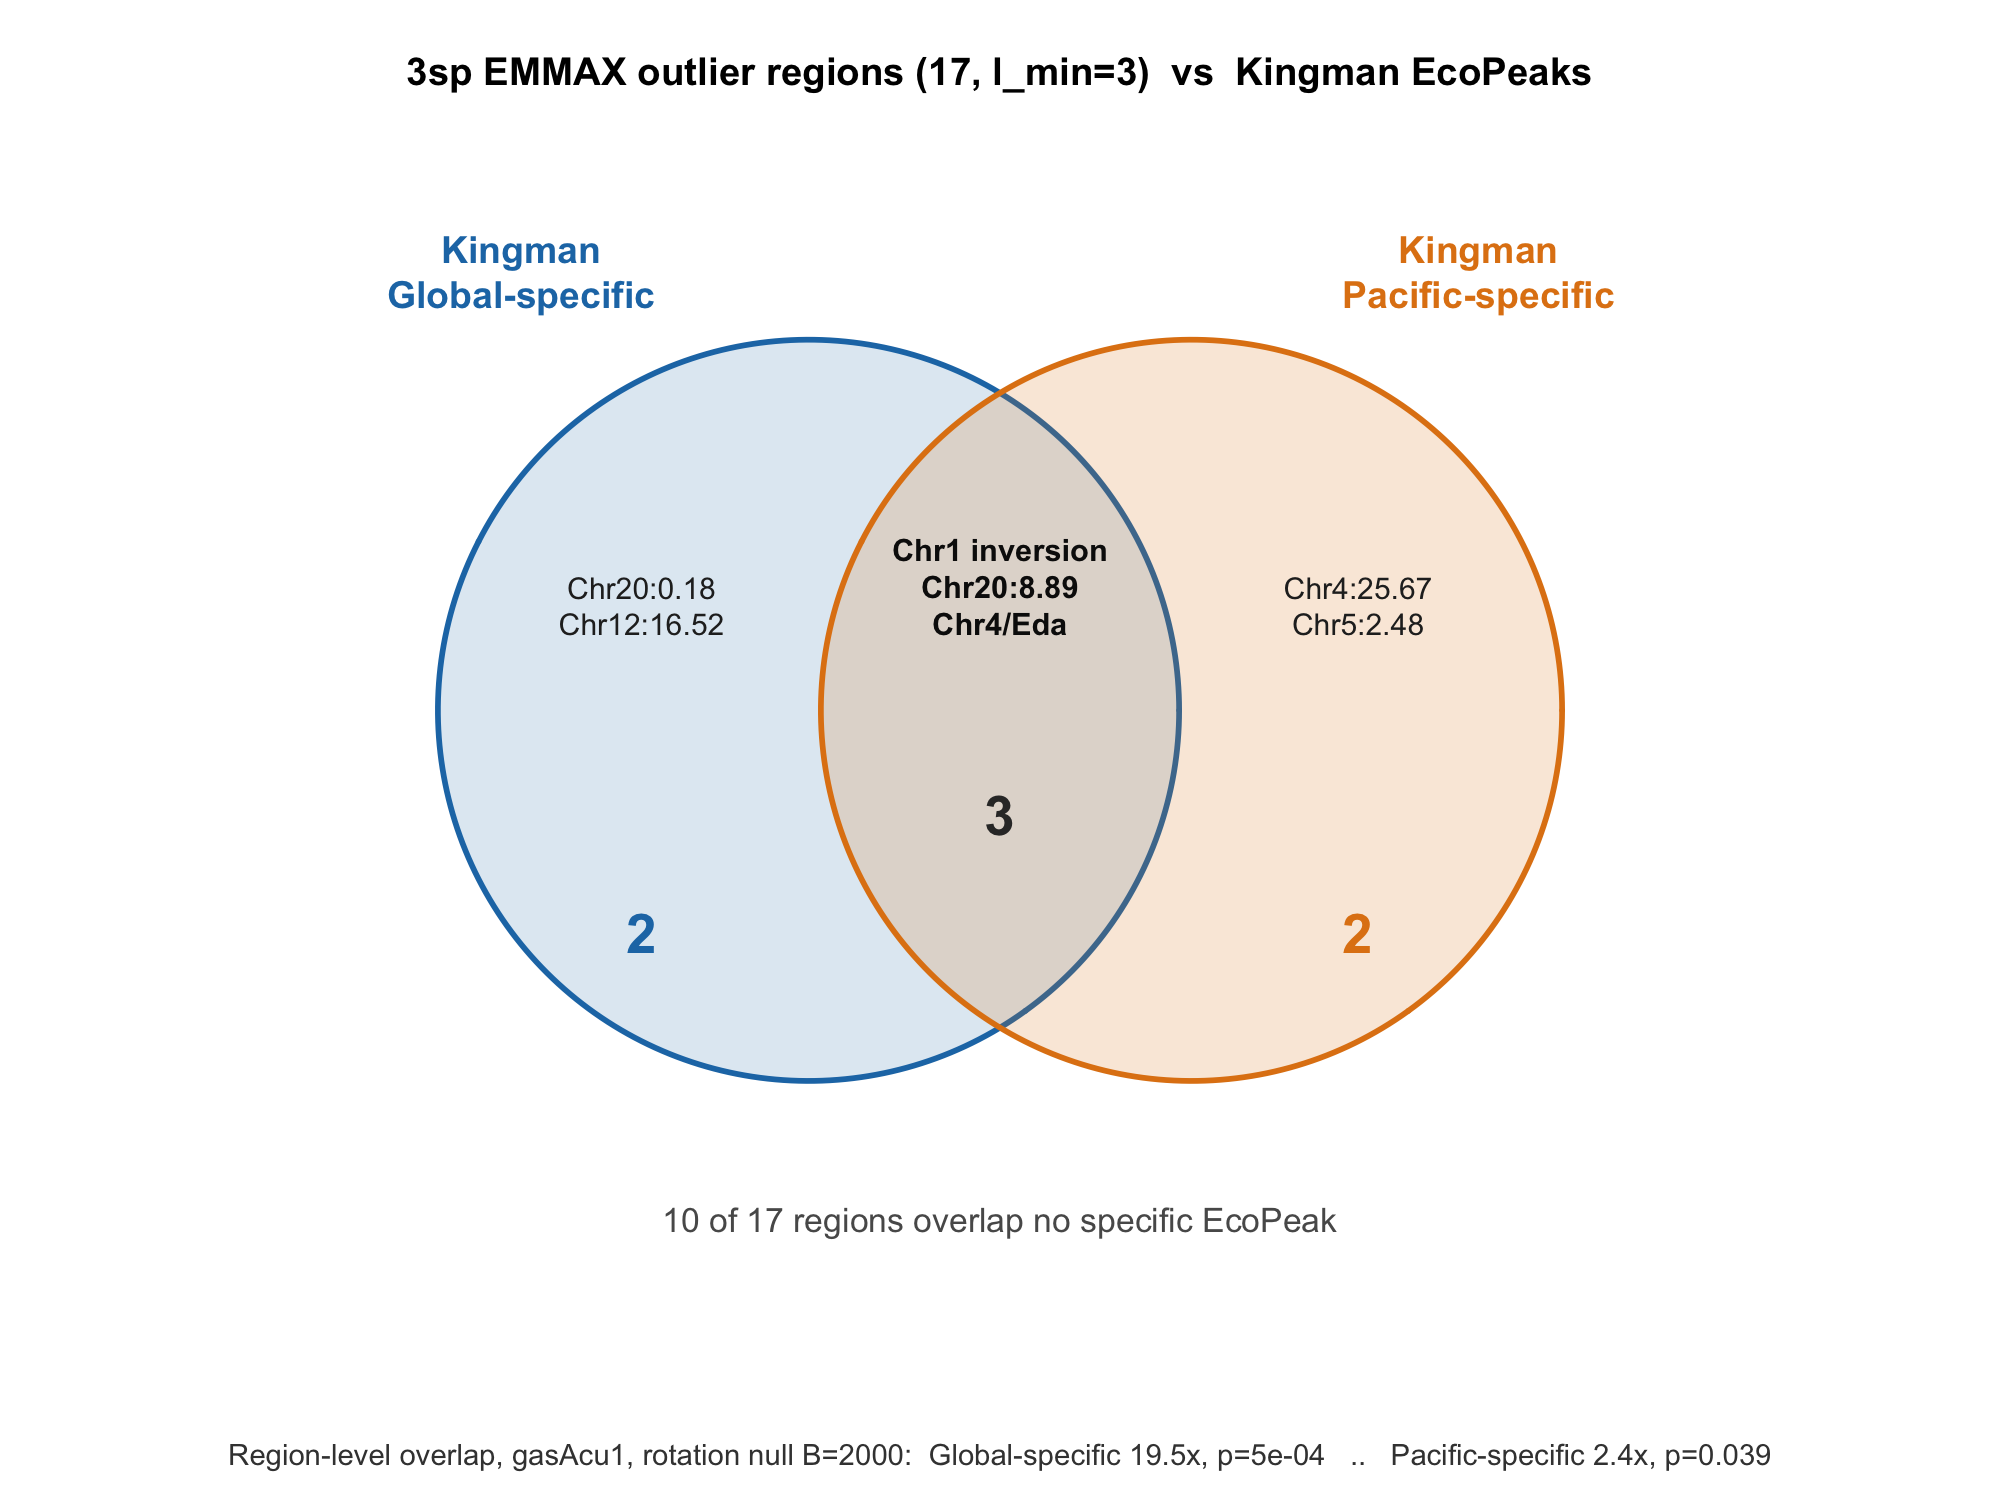
\includegraphics[width=0.78\linewidth]{fig5_venn_emmax17}
  \fbox{\parbox[c][0.30\linewidth][c]{\linewidth}{\centering\itshape
    Figure placeholder: Venn of the $17$ EMMAX outlier regions against the two
    Kingman \emph{specific} EcoPeak sets. Three regions---the chromosome-1
    inversion, \textit{Eda}, and chromosome-20 (8.9\,Mb)---fall in both cohorts;
    two are global-only, two Pacific-only, and ten overlap no specific EcoPeak.}}
  \caption{Overlap of the 3sp LD-aware outlier regions with the independently
  derived Kingman EcoPeaks.}
  \label{fig:venn}
\end{figure}

\section{Discussion}
\todo{Why region-level + consistency-score framing makes the null affordable and
is robust on saturated genomes; the detectability safeguard; limitations
(no self-calibration without a neutral floor); comparison to CSS / single-SNP
scans; outlook.}
\todo{Nuisance-structure estimation is the shared soft spot of both engines---LFMM
in its number of latent factors, EMMAX in how the GRM is estimated---so a scan is
only as trustworthy as its structure model. The $w_j$-pruned, $\lambda$-calibrated
kinship (Section~\ref{sec:grm}) turns the EMMAX side of this into a data-driven,
transferable choice rather than a hand-set one, and pairs with the structure-aware
null so the kinship need only avoid deflation. Empirically it excludes the
high-LD adaptive architecture on a real, LD-rich genome (the stickleback
inversions) while, on weak-LD simulations where the causal variants carry no local
LD, it harmlessly retains them and $\lambda$ recovers a kinship equivalent to the
complexity-reduction default---the same rule in both regimes. Caveat: $\lambda$
guards only against global deflation, so the $w_j$ axis, not $\lambda$, is what
forecloses regional signal absorption.}

\section{Supplementary: calibrating the kinship on the simulations}
\label{sec:supp-grm}

We validate the $\lambda \ge 1$ rule of Section~\ref{sec:grm} on the coalescent
simulations, where the causal variants are known and---because the simulated
genomes carry weak linkage---the QTN themselves have \emph{low} local LD, the
regime in which a permissive $w_j$ cutoff is most at risk of over-parameterising
the kinship. Sweeping the cutoff $\omega$ and reading off the genomic inflation
factor $\lambda$ (Table~\ref{tab:lambda-sweep}) shows $\lambda$ crossing one near
$\omega \approx 0.008$; the permissive ``below background LD'' cutoff
($\omega \approx b = 0.029$, retaining $96\%$ of markers) sits below one
($\lambda = 0.93$), i.e.\ deflated.

\begin{table}[h]
  \centering
  \begin{tabular}{lcc}
    \hline
    $w_j$ cutoff $\omega$ & markers kept & $\lambda$ \\
    \hline
    $0.006$          & $0.38$ & $1.19$ \\
    $0.008$          & $0.66$ & $1.04$ \\
    $0.010$          & $0.79$ & $1.00$ \\
    $0.014$          & $0.89$ & $0.97$ \\
    $0.020$          & $0.94$ & $0.95$ \\
    $0.028\,(\approx b)$ & $0.96$ & $0.93$ \\
    \hline
    complexity-reduction default & $0.35$ & $1.06$ \\
    \hline
  \end{tabular}
  \caption{Genomic inflation factor $\lambda$ and fraction of markers retained as
  the local-LD cutoff $\omega$ is tightened (mean over five environments,
  V2\_c1). $\lambda$ rises as the kinship is built from fewer, more independent
  markers, crossing one near $\omega \approx 0.008$. The complexity-reduction
  default reaches the same $\lambda \approx 1$ at a different marker count---%
  $\lambda$ calibrates the correction, not the number of markers.}
  \label{tab:lambda-sweep}
\end{table}

The $\lambda$-calibrated kinship ($\omega = 0.008$) matches the
complexity-reduction default on region-detection PR-AUC across region-size
filters $\ell_{\min}$ (Table~\ref{tab:grm-prauc}, within one standard error),
while the deflated below-background kinship trails by $0.05$--$0.08$, the gap
widest at small $\ell_{\min}$ where deflation costs recall. This confirms
empirically that (i) the failure of a permissive $w_j$ cutoff on weak-LD data is
\emph{global deflation}, not signal loss---the low-LD QTN are harmless in the
kinship, as argued in Section~\ref{sec:grm}---and (ii) tightening the cutoff to
$\lambda \ge 1$ recovers a kinship equivalent to the complexity-reduction default,
the same data-driven rule that yields the high-LD-excluding cutoff on the real
stickleback genome.

\begin{table}[h]
  \centering
  \begin{tabular}{lccccc}
    \hline
    kinship & $\lambda$ & $\ell_{\min}{=}1$ & $\ell_{\min}{=}2$ & $\ell_{\min}{=}4$ & $\ell_{\min}{=}8$ \\
    \hline
    complexity-reduction   & $1.06$ & $0.448$ & $0.453$ & $0.460$ & $0.397$ \\
    $w_j < 0.008$ ($\lambda{\approx}1$) & $1.04$ & $0.439$ & $0.464$ & $0.467$ & $0.433$ \\
    $w_j < b$ (deflated)   & $0.93$ & $0.369$ & $0.389$ & $0.412$ & $0.398$ \\
    \hline
  \end{tabular}
  \caption{Region-detection PR-AUC (mean over five environments, V2\_c1) under
  three EMMAX kinships, by region-size filter $\ell_{\min}$. The
  $\lambda$-calibrated $w_j$-pruned kinship matches the complexity-reduction
  default; the deflated below-background kinship ($\lambda = 0.93$) trails,
  especially at small $\ell_{\min}$.}
  \label{tab:grm-prauc}
\end{table}

\subsection{Cross-set corroboration of the stickleback outlier regions}
\label{sec:supp-crossset}

Table~\ref{tab:crossset} lists every consensus locus recovered by at least two of
six sets: the four 3sp scans---EMMAX and LFMM, each clustered at $\ell_{\min}=3$
(E3, L3) and $\ell_{\min}=10$ (E10, L10)---and the two Kingman \emph{specific}
EcoPeak sets (global, Glob; Pacific, Pac). Regions are merged across sets by overlap
(a $10$\,kb join tolerance) and ordered by how many sets recover them. Fifty-six
loci are shared by two or more sets; every EMMAX region and every $\ell_{\min}=10$
region is among them (none is a singleton), whereas $78$ of the $136$ LFMM
$\ell_{\min}=3$ regions are singletons recovered by no other set (final row). The
most secure loci head the table---the chromosome-1 inversion in all six columns,
Chr5:$2.5$ and Chr20:$0.18$ in five.

\begin{longtable}{lcccccc}
\caption{Consensus 3sp outlier loci recovered by $\ge 2$ of six sets. E3/E10: EMMAX
at $\ell_{\min}=3/10$; L3/L10: LFMM at $\ell_{\min}=3/10$; Glob/Pac: Kingman
global-/Pacific-specific EcoPeaks. A \checkmark\ marks a set with a region (or peak)
overlapping the locus. The final row counts regions unique to a single set.}
\label{tab:crossset}\\
\toprule
Locus (gasAcu1, Mb) & E3 & E10 & L3 & L10 & Glob & Pac \\
\midrule
\endfirsthead
\toprule
Locus (gasAcu1, Mb) & E3 & E10 & L3 & L10 & Glob & Pac \\
\midrule
\endhead
\midrule
\multicolumn{7}{r}{\footnotesize\emph{continued on next page}}\\
\endfoot
\midrule
\textit{unique (1 set only)} & $0$ & $0$ & $78$ & $0$ & --- & --- \\
\bottomrule
\endlastfoot
Chr1:21.07 (inversion) & \checkmark & \checkmark & \checkmark & \checkmark & \checkmark & \checkmark \\
Chr5:2.48 & \checkmark & \checkmark & \checkmark & \checkmark &  & \checkmark \\
Chr20:0.18 & \checkmark & \checkmark & \checkmark & \checkmark & \checkmark &  \\
Chr4:11.10 &  &  & \checkmark & \checkmark & \checkmark & \checkmark \\
Chr4:20.89 & \checkmark &  & \checkmark & \checkmark &  & \checkmark \\
Chr4:25.23 & \checkmark &  & \checkmark & \checkmark &  & \checkmark \\
Chr12:16.47 & \checkmark &  & \checkmark & \checkmark & \checkmark &  \\
Chr14:11.00 &  &  & \checkmark & \checkmark & \checkmark & \checkmark \\
Chr1:12.33 &  &  & \checkmark & \checkmark &  & \checkmark \\
Chr1:26.93 & \checkmark &  & \checkmark & \checkmark &  &  \\
Chr4:9.43 &  &  & \checkmark & \checkmark &  & \checkmark \\
Chr4:12.81 (Eda) & \checkmark &  &  &  & \checkmark & \checkmark \\
Chr4:14.03 &  &  & \checkmark & \checkmark &  & \checkmark \\
Chr4:26.49 & \checkmark &  & \checkmark & \checkmark &  &  \\
Chr7:11.55 & \checkmark & \checkmark & \checkmark &  &  &  \\
Chr7:17.99 &  &  & \checkmark &  & \checkmark & \checkmark \\
Chr8:9.26 &  &  & \checkmark &  & \checkmark & \checkmark \\
Chr11:0.00 &  &  & \checkmark & \checkmark &  & \checkmark \\
Chr11:6.11 &  &  & \checkmark & \checkmark &  & \checkmark \\
Chr11:8.86 &  &  & \checkmark &  & \checkmark & \checkmark \\
Chr12:11.75 &  &  & \checkmark & \checkmark &  & \checkmark \\
Chr12:15.55 & \checkmark &  & \checkmark & \checkmark &  &  \\
Chr16:11.54 &  &  & \checkmark & \checkmark &  & \checkmark \\
Chr16:16.48 &  &  & \checkmark & \checkmark &  & \checkmark \\
Chr17:6.45 & \checkmark &  & \checkmark & \checkmark &  &  \\
Chr17:9.94 & \checkmark &  & \checkmark & \checkmark &  &  \\
Chr18:0.80 &  &  & \checkmark & \checkmark &  & \checkmark \\
Chr18:5.61 & \checkmark &  & \checkmark & \checkmark &  &  \\
Chr20:8.89 & \checkmark &  &  &  & \checkmark & \checkmark \\
Chr21:7.00 &  &  & \checkmark &  & \checkmark & \checkmark \\
Chr1:8.87 &  &  & \checkmark &  &  & \checkmark \\
Chr2:9.43 &  &  & \checkmark & \checkmark &  &  \\
Chr2:22.52 &  &  & \checkmark & \checkmark &  &  \\
Chr3:3.76 &  &  & \checkmark & \checkmark &  &  \\
Chr3:6.72 &  &  & \checkmark & \checkmark &  &  \\
Chr3:13.03 & \checkmark &  & \checkmark &  &  &  \\
Chr4:24.72 &  &  & \checkmark &  &  & \checkmark \\
Chr5:1.55 &  &  & \checkmark & \checkmark &  &  \\
Chr6:1.40 &  &  & \checkmark & \checkmark &  &  \\
Chr7:0.06 &  &  & \checkmark & \checkmark &  &  \\
Chr7:6.95 &  &  & \checkmark &  &  & \checkmark \\
Chr7:10.53 &  &  & \checkmark & \checkmark &  &  \\
Chr7:14.49 &  &  & \checkmark &  &  & \checkmark \\
Chr8:0.11 &  &  & \checkmark & \checkmark &  &  \\
Chr8:1.45 &  &  & \checkmark & \checkmark &  &  \\
Chr8:5.52 &  &  & \checkmark &  &  & \checkmark \\
Chr8:10.33 &  &  & \checkmark & \checkmark &  &  \\
Chr10:6.24 &  &  & \checkmark & \checkmark &  &  \\
Chr11:11.99 &  &  & \checkmark & \checkmark &  &  \\
Chr12:2.48 &  &  & \checkmark & \checkmark &  &  \\
Chr14:14.94 &  &  & \checkmark & \checkmark &  &  \\
Chr16:4.23 &  &  & \checkmark & \checkmark &  &  \\
Chr20:2.21 &  &  & \checkmark & \checkmark &  &  \\
Chr20:3.67 & \checkmark &  & \checkmark &  &  &  \\
Chr20:6.25 &  &  & \checkmark &  &  & \checkmark \\
Chr21:2.18 &  &  & \checkmark &  &  & \checkmark \\
\end{longtable}

\bibliographystyle{plainnat}
\bibliography{references}

\end{document}
